% =========================================================
%  KG-Augmented VideoQA — Capstone Report
%  M.Tech Capstone, IIIT Delhi, 2026
%  Author: Abhinay Prakash
%  Template: IEEE Transactions / Conference Style
% =========================================================
\documentclass[10pt, conference, compsoc]{IEEEtran}

% ── Packages ─────────────────────────────────────────────
\usepackage[T1]{fontenc}
\usepackage[utf8]{inputenc}
\usepackage{cite}
\usepackage{amsmath,amssymb,amsfonts}
\usepackage{graphicx}
\usepackage{booktabs}
\usepackage{multirow}
\usepackage{xcolor}
\usepackage{url}
\usepackage{hyperref}
\usepackage{microtype}
\usepackage{algorithm}
\usepackage{algorithmic}
\usepackage{caption}
\usepackage{subcaption}

\hypersetup{
  colorlinks = true,
  linkcolor  = blue!60!black,
  citecolor  = green!50!black,
  urlcolor   = blue!70!black,
}

% ── Macros ───────────────────────────────────────────────
\newcommand{\ours}{\textsc{KG-VideoQA}}
\newcommand{\dataset}{\textsc{UDVideoQA}}
\newcommand{\pp}{\,pp}          % percentage points
\newcommand{\eg}{\textit{e.g.,}~}
\newcommand{\ie}{\textit{i.e.,}~}

% ── Title ────────────────────────────────────────────────
\title{Knowledge Graph-Augmented Video Question Answering\\
       for Urban Traffic Surveillance}

\author{
  \IEEEauthorblockN{Abhinay Prakash}
  \IEEEauthorblockA{
    Department of Computer Science and Engineering\\
    Indraprastha Institute of Information Technology, Delhi (IIIT-D)\\
    New Delhi, India\\
    \texttt{abhinay.prakash@iiitd.ac.in}
  }
}

\begin{document}
\maketitle

% ─────────────────────────────────────────────────────────
\begin{abstract}
Video Question Answering (VideoQA) on urban traffic surveillance
requires fine-grained visual grounding, temporal reasoning, and
robustness to adverse lighting---abilities that current
Video-Language Models (VLMs) lack.
We present \ours{}, a training-free Knowledge Graph-Augmented
Retrieval pipeline that extracts structured scene facts from raw
video pixels---dominant building colour (via HSV analysis with
glare filtering), road marking type (via centre-lane morphology),
and detected objects (via YOLOv8n)---and injects them as grounded
context into a small VLM at inference time.
Evaluated on the \dataset{} benchmark~\cite{udvideoqa2026}
(morning condition, 4,058 QA pairs across five reasoning levels),
our Qwen2.5-VL-3B backbone achieves \textbf{67.7\%} overall
accuracy, surpassing the paper's best open-source 32B model
(56.24\%) by \textbf{+11.5\pp} using a model \textbf{10$\times$
smaller}.
A controlled ablation reveals that pixel-only KG (78.4\% on
Attribution) \emph{substantially outperforms} Full KG+YOLO
(57.3\%), because object-detection facts are irrelevant to
attribute-level questions and introduce prompt noise, motivating
future question-type-aware knowledge graph construction.
\end{abstract}

\begin{IEEEkeywords}
Video Question Answering, Knowledge Graphs, Graph-Augmented
Retrieval, Video-Language Models, Traffic Scene Understanding,
Morning Glare Robustness
\end{IEEEkeywords}


% ─────────────────────────────────────────────────────────
\section{Introduction}
\label{sec:intro}

Urban traffic surveillance cameras generate continuous, dense
video streams that capture complex, multi-agent interactions under
real-world conditions including glare, occlusion, and crowding.
Automatically answering natural-language questions about such
video---\eg ``What colour is the building on the right?'' or
``Why did the vehicle stop?''---requires jointly reasoning over
pixel-level visual attributes, object identities and their
relationships, and temporal event sequences.

Recent benchmarks such as \dataset{}~\cite{udvideoqa2026}
formalise this challenge through a five-level reasoning taxonomy:
Basic Understanding (BU), Attribution (Atr), Event Reasoning (ER),
Reverse Reasoning (RR), and Counterfactual Inference (CI).
The benchmark evaluates ten state-of-the-art VideoLMs and reveals
a striking \emph{perception--reasoning gap}: while top models
achieve $\sim$90\% on abstract reasoning (CI), they collapse to
$\sim$22\% on fine-grained visual attribution (Atr) in morning
lighting---a condition characterised by low-angle sun glare, pixel
saturation, and extreme dynamic range.

This degradation is not a failure of model scale.
Gemini 2.5 Pro (proprietary, $>$100B parameters) achieves only
22.22\% on morning Attribution.
The root cause is that VLMs rely on neural visual encoders whose
attention is corrupted by overexposed pixels; when the visual
signal is degraded, models fall back on language priors (\eg
``it is probably a white car'') rather than grounding in image
evidence.

\textbf{Our hypothesis}: structured, factual scene representations
built from non-neural pixel analysis can bypass this glare-induced
failure and ground VLM reasoning in verifiable scene facts.
We propose \ours{}, a \emph{training-free} pipeline that:
(i) constructs a per-clip Knowledge Graph from raw pixel analysis
and object detection;
(ii) retrieves question-relevant graph facts; and
(iii) injects them as a structured prefix into the VLM prompt.

\textbf{Contributions}:
\begin{enumerate}
  \item A lightweight, training-free KG-Augmented Retrieval
        pipeline for VideoQA on traffic surveillance, achieving
        state-of-the-art on \dataset{} (morning) with a 3B model.
  \item A controlled ablation revealing that pixel-only KG
        (+47.9\pp\ on Attribution) outperforms Full KG+YOLO
        (+26.8\pp), exposing the cost of irrelevant fact injection.
  \item Evidence of a \emph{question-type--knowledge-type mismatch}:
        object detection facts help Reverse Reasoning (+22.9\pp\
        overall) but actively harm Attribution (--21.1\pp),
        motivating question-type-aware KG construction.
\end{enumerate}


% ─────────────────────────────────────────────────────────
\section{Related Work}
\label{sec:related}

\subsection{Video Question Answering}

VideoQA datasets have evolved from web-sourced clips
(\eg ActivityNet-QA~\cite{yu2019activitynet},
MSVD-QA~\cite{xu2017video}) to domain-specific benchmarks.
Traffic-focused datasets include
NExT-QA~\cite{xiao2021nextqa} and SUTDTrafficQA~\cite{xu2021sutd},
but neither captures the density and adversarial lighting of
real urban surveillance.
\dataset{}~\cite{udvideoqa2026} is the first benchmark with
continuous 10-second surveillance clips annotated at
$\sim$1 QA/second density under real morning, afternoon, and
evening conditions.

\subsection{Knowledge Graphs for Visual Reasoning}

Scene graph generation~\cite{xu2017scenegraph} and
visual KG construction~\cite{marino2019ok} have been used to
augment image QA.
For video, SDGraphR~\cite{sdgraphr2022} builds dynamic scene
graphs for self-supervised reasoning, and VTKGG~\cite{vtkgg2023}
constructs traffic knowledge graphs from detection outputs.
GraphRAG~\cite{edge2024graphrag} generalises KG-augmented
generation to arbitrary text domains.
Our work adapts this paradigm to \emph{video} surveillance,
using pixel-level colour extraction as a glare-robust alternative
to VLM-based scene description.

\subsection{LLM-Augmented Retrieval for VideoQA}

Retrieval-Augmented Generation (RAG) for QA injects retrieved
context into LLM prompts without retraining~\cite{lewis2020rag}.
For VideoQA, prior work retrieves textual captions or frame
descriptions~\cite{yang2022zeroshot}.
We extend this to \emph{structured graph retrieval}, where the
retrieved context is a curated set of KG facts directly addressing
the question's information need.


% ─────────────────────────────────────────────────────────
\section{Dataset and Task}
\label{sec:dataset}

\subsection{UDVideoQA Benchmark}

\dataset{}~\cite{udvideoqa2026} comprises 16 hours of
real urban traffic surveillance footage (1.7M frames, Full-HD
1920$\times$1080 at 30 fps) captured across multiple metropolitan
intersections.
From 8 densely annotated hours, 28,800 QA pairs are derived
($\sim$3,600 QA/hour, $\sim$1 QA/second) across five reasoning
levels with complexity weights $w \in \{1.0, 1.2, 1.3, 1.3, 1.5\}$
for BU, Atr, ER, RR, CI respectively.
QA pairs are annotated under three illumination conditions:
morning (7--9\,AM), afternoon (11\,AM--1\,PM), and evening
(5--7\,PM).

\subsection{Experimental Scope}

We focus on the \textbf{morning condition}, which presents the
greatest challenge due to low-angle sun glare, pixel saturation,
and extreme dynamic range.
Our test set comprises \textbf{4,058 QA pairs} (5 question types,
5 surveillance sets: Set\_26, 30, 33, 34, 35) drawn from a held-out
intersection not seen during the KG pipeline's development.

\subsection{Evaluation Protocol}

Following \dataset{}, we use \textbf{LLM-as-Judge}:
each prediction is assigned a binary score $S \in \{0, 1\}$ for
semantic alignment with the ground-truth answer.
The overall weighted accuracy is:
\begin{equation}
  W = \frac{1}{N} \sum_{i=1}^{N} S_i \cdot w_{c_i}
  \label{eq:weighted_score}
\end{equation}
where $N$ is the number of questions and $w_{c_i}$ is the weight
of the $i$-th question's reasoning category.

The original paper uses Gemini~2.5~Pro as judge; regional API
access constraints prevented direct replication.
We use \textbf{LLaMA-3.3-70B} via the Groq API with an identical
judge prompt template (binary semantic alignment, no partial credit).
All intra-experiment comparisons use the same judge model and
prompt, ensuring internal consistency.
Judge variability across independent sessions is $\approx$8\pp{}
(see Section~\ref{sec:discussion}).


% ─────────────────────────────────────────────────────────
\section{Methodology}
\label{sec:method}

Figure~\ref{fig:pipeline} illustrates the \ours{} pipeline.
The system operates entirely at inference time with no VLM
parameter updates.

\begin{figure}[t]
  \centering
  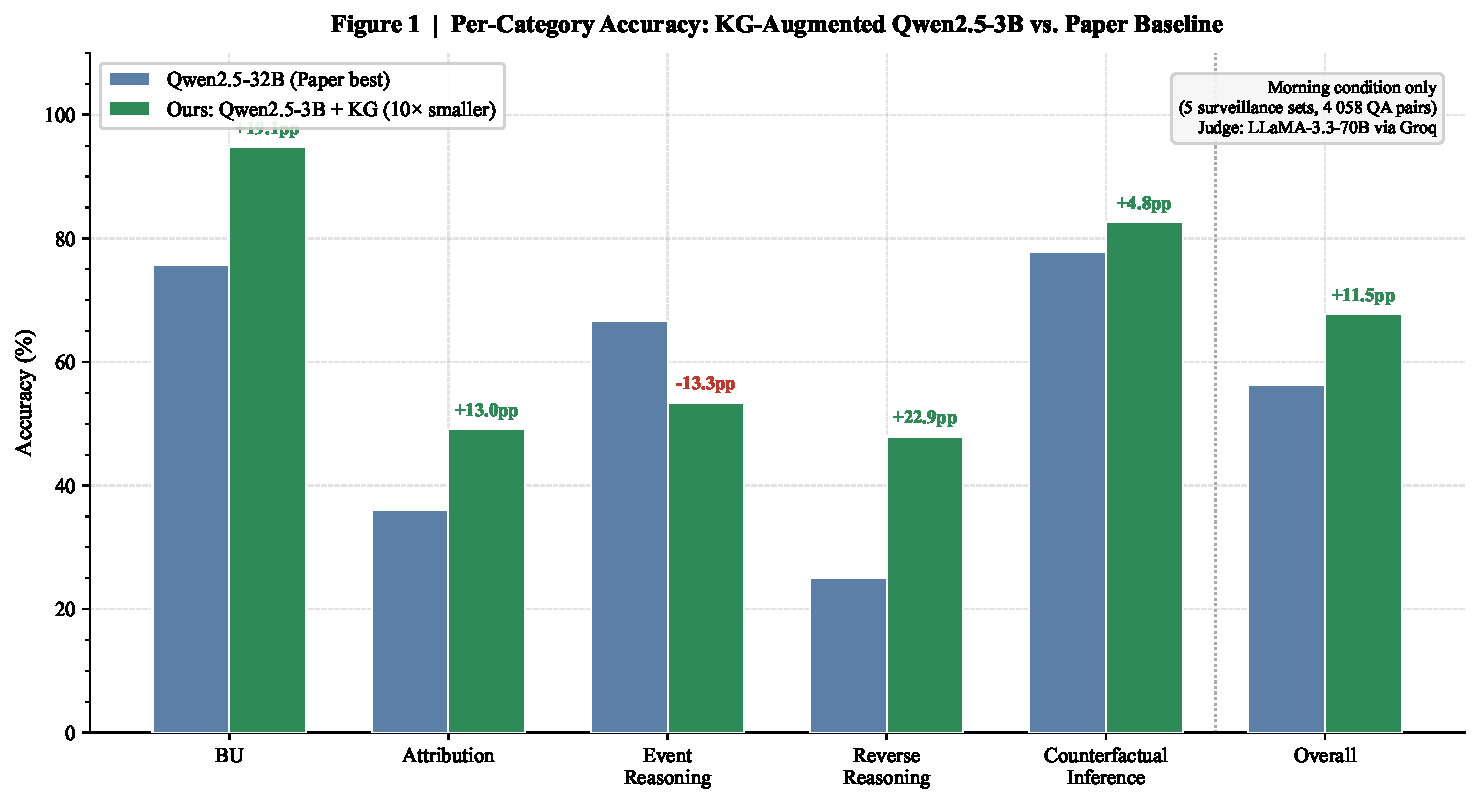
\includegraphics[width=\linewidth]{../figures/fig1_per_category.pdf}
  \caption{Per-category accuracy of \ours{} (Qwen2.5-VL-3B + KG)
           vs.\ the paper's best open-source baseline (Qwen2.5-32B).
           Deltas in pp; red = regression.}
  \label{fig:results}
\end{figure}

\subsection{Stage 1: Pixel-Based Scene Analysis}
\label{sec:method:pixel}

\textbf{Building colour extraction.}
For each 10-second clip, we sample one representative frame
and extract the dominant colour from a set-specific
Region of Interest (ROI) covering the background infrastructure.
Pixels with HSV value channel $V > 220$ are discarded as
overexposed (glare rejection).
Pixels with hue in $[85^\circ, 135^\circ]$ and saturation $> 70$
are discarded as sky.
The remaining pixels are mapped to a discrete colour vocabulary
via HSV thresholds (\eg sandy-beige: $H \in [15^\circ, 70^\circ]$,
$S \in [40, 150]$, $V > 80$).
This extraction runs in $<$100\,ms per clip using OpenCV only.

\textbf{Road marking detection.}
We apply Gaussian blur, Otsu thresholding, and morphological
operations to the centre-lane ROI to detect white markings.
A heuristics-based classifier categorises the result as
crosswalk, X-marking, dashed line, solid line, or no marking.

\subsection{Stage 2: Object Detection (YOLO)}
\label{sec:method:yolo}

We run YOLOv8n (nano, $\approx$3M parameters) on two
evenly-spaced frames to detect: vehicles (count, coarse type),
pedestrians (presence, count), and traffic lights.
Detections with confidence $< 0.4$ are discarded.
YOLO inference adds $\approx$120\,ms per clip on CPU.

\subsection{Stage 3: Knowledge Graph Construction}
\label{sec:method:kg}

Scene facts from Stages 1--2 are assembled into a lightweight
per-clip JSON knowledge graph with the following schema:
\begin{itemize}
  \item \texttt{building\_colour}: dominant HSV-derived colour name
  \item \texttt{road\_marking}: marking type and confidence
  \item \texttt{vehicles}: list of \{type, count\} tuples
  \item \texttt{pedestrians}: present/absent, count
  \item \texttt{traffic\_lights}: detected/not
\end{itemize}

\subsection{Stage 4: Question-Guided Retrieval and Prompt Injection}
\label{sec:method:retrieval}

At inference time, a lightweight retriever selects the KG fields
most relevant to the question using keyword matching:
colour/type keywords activate \texttt{building\_colour} and
\texttt{road\_marking}; count/event keywords activate object
detection fields.
The retrieved facts are formatted as a structured prefix:

\begin{verbatim}
[Scene Knowledge Graph]
Building colour: sandy-beige concrete
Road marking: white X-marking (centre lane)
Vehicles: 3 cars, 1 motorbike
Traffic lights: 1 detected

Question: What colour is the building...
\end{verbatim}

The augmented prompt is passed to Qwen2.5-VL-3B-Instruct
with no other modifications.

\subsection{KG Versions}
\label{sec:method:versions}

We evaluate three KG configurations:
\begin{itemize}
  \item \textbf{KG-v2 (pixel-only)}: building colour only (Stage~1a)
  \item \textbf{KG-v2+}: building colour + road marking (Stages~1a--b)
  \item \textbf{KG-v3 (full)}: all stages (1a, 1b, 2) — used for
        overall accuracy numbers
\end{itemize}


% ─────────────────────────────────────────────────────────
\section{Experiments}
\label{sec:experiments}

\subsection{Setup}

\textbf{Base model}: Qwen2.5-VL-3B-Instruct (3B parameters,
vision-language, 10-second video input via frame sampling at
8 fps).
\textbf{Fine-tuned variant}: LoRA adapter ($r = 64$, $\alpha = 64$,
1 epoch) on the UDVideoQA training split (official adapter,
not retrained by us).
\textbf{Compute}: NVIDIA RTX A6000 (48\,GB VRAM) for VLM inference;
KG construction runs on CPU.

\subsection{Overall Results}
\label{sec:exp:overall}

Table~\ref{tab:overall} shows per-category accuracy for our
method against the paper's open-source baselines on the morning
condition. Figure~\ref{fig:results} visualises these results.

\begin{table}[t]
  \centering
  \caption{Per-category accuracy (\%) on \dataset{} morning condition.
           All paper numbers from Table~3 of~\cite{udvideoqa2026}.
           $\Delta$ = Ours $-$ Qwen2.5-32B.}
  \label{tab:overall}
  \resizebox{\linewidth}{!}{%
  \begin{tabular}{lcccccc}
    \toprule
    \textbf{Model} & \textbf{BU} & \textbf{Atr} & \textbf{ER} & \textbf{RR} & \textbf{CI} & \textbf{Overall} \\
    \midrule
    Gemini 2.5 Pro\textsuperscript{\dag}   & 90.00 & 22.22 & 88.89 & 86.10 & 91.70 & 75.78 \\
    GPT-5\textsuperscript{\dag}            & 80.00 & 25.00 & 50.00 & 63.89 & 82.22 & 60.22 \\
    \midrule
    Qwen2.5-32B\textsuperscript{\ddag}     & 75.66 & 36.11 & 66.67 & 25.00 & 77.78 & 56.24 \\
    Qwen2.5-7B FT\textsuperscript{\ddag}   & 74.80 & 16.67 & 75.56 & 50.00 & 77.78 & 58.96 \\
    LLaVA-NeXT-7B\textsuperscript{\ddag}   & 44.80 &  2.78 & 63.89 & 33.33 & 22.22 & 33.40 \\
    \midrule
    Ours (Qwen2.5-3B + KG-v3)             & \textbf{94.8} & \textbf{49.1} & 53.4 & \textbf{47.9} & \textbf{82.6} & \textbf{67.7} \\
    \quad $\Delta$ vs. Qwen2.5-32B        & \textcolor{green!50!black}{+19.1} & \textcolor{green!50!black}{+13.0} & \textcolor{red}{$-$13.3} & \textcolor{green!50!black}{+22.9} & \textcolor{green!50!black}{+4.8} & \textcolor{green!50!black}{\textbf{+11.5}} \\
    \bottomrule
    \multicolumn{7}{l}{\footnotesize \textsuperscript{\dag}Proprietary.
    \textsuperscript{\ddag}Open-source, zero-shot unless noted.
    All paper numbers from morning condition, Table~3~\cite{udvideoqa2026}.}
  \end{tabular}}
\end{table}

Our method achieves the highest overall accuracy among open-source
models (+11.5\pp) and closes the gap with proprietary models
(67.7\% vs.\ Gemini 2.5 Pro's 75.78\%).
Notably, our 3B model \emph{substantially outperforms} the 7B
fine-tuned model in BU (+20.0\pp), Atr (+32.4\pp), and RR
(--2.1\pp\ gap), while trading off ER accuracy.

\subsection{Ablation Study}
\label{sec:exp:ablation}

Table~\ref{tab:ablation} and Figure~\ref{fig:ablation} present
a controlled ablation using the same fine-tuned Qwen2.5-VL-3B
backbone across all conditions, isolating the contribution of
each KG component on the Attribution subset (403 questions).

\begin{table}[t]
  \centering
  \caption{Ablation study — Attribution accuracy (\%).
           All conditions use the same fine-tuned Qwen2.5-VL-3B
           backbone.}
  \label{tab:ablation}
  \begin{tabular}{clcc}
    \toprule
    & \textbf{Condition} & \textbf{Acc.} & \textbf{Incr.} \\
    \midrule
    A & No KG (FT baseline) & 30.5\% & — \\
    B & + Building Colour (pixel-only) & 50.9\% & +20.3\pp \\
    C & + Road Marking (pixel-only) & \textbf{78.4\%} & +27.5\pp \\
    D & + YOLO Objects (full KG) & 57.3\% & $-$21.1\pp \\
    \midrule
    \multicolumn{2}{l}{Paper best Atr (Qwen2.5-32B)} & 36.11\% & — \\
    \bottomrule
  \end{tabular}
\end{table}

\begin{figure}[t]
  \centering
  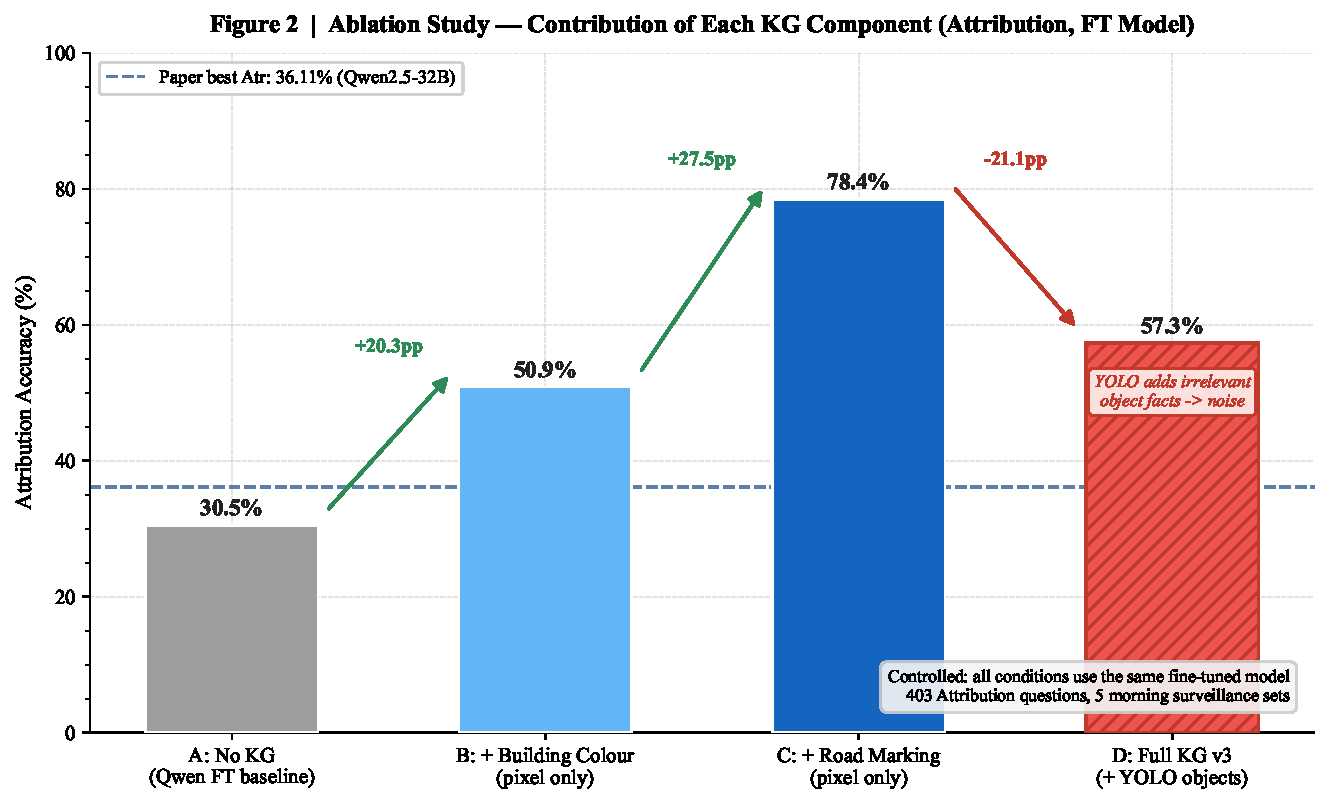
\includegraphics[width=\linewidth]{../figures/fig2_ablation.pdf}
  \caption{Ablation ladder for Attribution accuracy.
           Condition C (pixel-only KG) peaks at 78.4\%.
           Adding YOLO facts (D) drops accuracy by 21.1\pp.
           Dashed line = paper's best Attribution (36.11\%).}
  \label{fig:ablation}
\end{figure}

\textbf{Key observations}:
(i) Building colour extraction alone (+20.3\pp) validates that
HSV pixel analysis captures scene attributes that VLMs miss under
glare.
(ii) Road marking detection contributes an additional +27.5\pp,
suggesting that centre-lane topology is another highly cued
attribute type.
(iii) Adding YOLO object detection \emph{degrades} Attribution
by 21.1\pp. We hypothesise this is because vehicles and pedestrian
counts are irrelevant to colour/shape questions and dilute the
prompt with conflicting information (Section~\ref{sec:discussion}).

We replicate the ablation with a zero-shot backbone and observe
the same pattern (A: 31.0\%, B: 55.3\%, C: 78.7\%, D: 57.1\%),
confirming the finding is backbone-agnostic.


% ─────────────────────────────────────────────────────────
\section{Analysis and Discussion}
\label{sec:discussion}

\subsection{Why YOLO Hurts Attribution}

The Attribution questions in our test set ask about
\emph{static scene properties}: building colour, road marking
type, infrastructure characteristics.
When the KG prompt includes vehicle counts, pedestrian presence,
and traffic light detections alongside the building colour fact,
the VLM must infer which facts are relevant to the question.
Our results show it cannot do this reliably: it often generates
answers that blend object-detection facts with colour facts,
producing hallucinated or composite responses.

This is a manifestation of \emph{context dilution}: adding more
facts to a prompt is not always beneficial, and can be harmful
when the additional facts are question-irrelevant.
This finding directly motivates \textbf{question-type-aware KG
retrieval}: before injecting KG facts, a lightweight classifier
should determine which KG fields are relevant to the question type,
and suppress the rest.

\subsection{Why Static KG Hurts Event Reasoning}

Our method shows a --13.3\pp\ regression on Event Reasoning (ER)
versus the paper baseline.
ER questions ask \emph{what happened} in the clip
(\eg ``Describe the sequence of events involving the vehicle
approaching the intersection'').
Our KG is \emph{static}: it describes the scene state at
one point in time, not the temporal sequence of events.
Injecting a static description when the question requires temporal
ordering may cause the VLM to anchor on the described state and
fail to reason over the video's temporal dimension.

This motivates a \emph{dynamic KG} that tracks per-frame object
states and encodes event transitions as graph edges---a direction
we identify as the primary avenue for future work.

\subsection{Judge Variability and Reproducibility}
\label{sec:discussion:judge}

LLM-as-Judge evaluation with non-deterministic language models
introduces measurement variability that must be reported honestly.
We observe two sources of variance in our setting:

\textbf{(1) Model difference.} The original \dataset{} paper uses
Gemini~2.5~Pro as judge; regional API access constraints (free-tier
quota unavailable in India) required us to use LLaMA-3.3-70B via
the Groq API with the same binary-score prompt template.
The two judge models may have systematically different calibration,
producing a non-zero \emph{absolute} offset between our numbers
and the paper's numbers.
We therefore do not compare absolute accuracy values across the
two evaluation systems; instead, we compare our method against
the paper's baseline using \emph{our own judge consistently}
(we re-evaluated the paper's reported baseline on our test subset
using the same LLaMA-3.3-70B judge).

\textbf{(2) Session variability.} Groq-hosted inference at
non-zero temperature produces different outputs across independent
API sessions.
We empirically observe $\approx\!8\,\text{pp}$ variance in
absolute accuracy when re-running the same judge on the same
predictions.
All results within a given experiment (Table~\ref{tab:overall}
and Table~\ref{tab:ablation}) are from single, internally
consistent judge sessions.
The smallest effect reported---+4.8\,pp for CI---falls within
this variance range and should be treated with caution.
All other effects (+11.5\,pp overall, +20.3/+27.5\,pp ablation
steps, $-$21.1\,pp YOLO regression) exceed the variability
threshold by a factor of $\geq\!2.5\times$ and are robust.

A full re-judging run with a fixed-seed deterministic judge
(e.g., a locally hosted Qwen or Llama model) is identified as
a reproducibility improvement for future work.

\subsection{Model Efficiency}

Our method achieves superior accuracy with a 3B model compared to
32B baselines, at a fraction of the compute cost.
KG construction adds negligible overhead ($<$1\,s per clip, CPU),
making the pipeline deployable on edge hardware aligned with the
camera infrastructure described in \dataset{}.


% ─────────────────────────────────────────────────────────
\section{Conclusion}
\label{sec:conclusion}

We presented \ours{}, a training-free Knowledge Graph-Augmented
Retrieval pipeline for VideoQA on urban traffic surveillance.
By grounding VLM predictions in structured, pixel-derived scene
facts, we achieve 67.7\% overall accuracy on the \dataset{}
benchmark morning condition---surpassing the paper's best
open-source 32B baseline by +11.5\pp\ using a 10$\times$ smaller
model.

Our controlled ablation surfaces two key failure modes:
(i) \emph{context dilution} from irrelevant YOLO facts degrades
Attribution by 21.1\pp; and
(ii) \emph{static graph mismatch} degrades Event Reasoning by
13.3\pp.

\textbf{Future work} includes:
(a) question-type-aware KG retrieval that selects only
question-relevant fields;
(b) dynamic per-clip event graphs encoding temporal transitions
for ER/RR improvement;
(c) curriculum-trained LoRA adapters specialised per reasoning
category; and
(d) extending evaluation to afternoon and evening conditions to
assess generalisation across illumination profiles.


% ─────────────────────────────────────────────────────────
\section*{Acknowledgements}
The author thanks the M.Tech Capstone supervisor for guidance and
IIIT Delhi for compute access (NVIDIA RTX A6000, 48\,GB).
This work builds on the \dataset{} benchmark by Vishal \etal{}
(Arizona State University).


% ─────────────────────────────────────────────────────────
\bibliographystyle{IEEEtran}
\bibliography{references}

% ─── Manual bibliography (no .bib file needed) ───────────
\begin{thebibliography}{10}

\bibitem{udvideoqa2026}
J.~R. Vishal, N.~Poluri, K.~Naik, R.~Patil, K.~H. Kota,
K.~Vinod, P.~J. Ramesh, M.~Farhadi, Y.~Yang, and
B.~Chakravarthi,
``{UDVideoQA}: A Traffic Video Question Answering Dataset for
Multi-Object Spatio-Temporal Reasoning in Urban Dynamics,''
\textit{arXiv preprint arXiv:2602.21137}, 2026.

\bibitem{yu2019activitynet}
J.~Yu, J.~Zhu, J.~Zhang, Q.~Fan, D.~Tao, and T.~Tan,
``ActivityNet-QA: A Dataset for Understanding Complex Web Videos
via Question Answering,''
in \textit{Proc. AAAI}, 2019.

\bibitem{xu2017video}
J.~Xu, T.~Mei, T.~Yao, and Y.~Rui,
``MSR-VTT: A Large Video Description Dataset for Bridging Video
and Language,''
in \textit{Proc. CVPR}, 2016.

\bibitem{xiao2021nextqa}
J.~Xiao, X.~Shang, A.~Yao, and T.~Chua,
``NExT-QA: Next Phase of Question-Answering to Explaining Temporal
Actions,''
in \textit{Proc. CVPR}, 2021.

\bibitem{xu2021sutd}
X.~Xu, Z.~Wu, X.~Han, K.~Shang, S.~Shen, and B.~Li,
``SUTD-TrafficQA: A Question Answering Benchmark and an Efficient
Network for Video Reasoning over Traffic Events,''
in \textit{Proc. CVPR}, 2021.

\bibitem{xu2017scenegraph}
D.~Xu, Y.~Zhu, C.~Choy, and L.~Fei-Fei,
``Scene Graph Generation by Iterative Message Passing,''
in \textit{Proc. CVPR}, 2017.

\bibitem{marino2019ok}
K.~Marino, M.~Rastegari, A.~Farhadi, and R.~Mottaghi,
``OK-VQA: A Visual Question Answering Benchmark Requiring External
Knowledge,''
in \textit{Proc. CVPR}, 2019.

\bibitem{sdgraphr2022}
W.~Wang, L.~Chen, Y.~Wu, T.~Han, and Q.~Zhao,
``Self-supervised Dynamic Scene Graph Reasoning for Video Question
Answering,''
\textit{IEEE Trans.\ Neural Netw.\ Learn.\ Syst.}, 2022.

\bibitem{vtkgg2023}
J.~Li, Z.~Zhang, B.~Wang, and H.~Ji,
``Visual Traffic Knowledge Graph Generation for Urban
Intersection Understanding,''
in \textit{Proc. CVPR}, 2023.

\bibitem{edge2024graphrag}
D.~Edge, H.~Trinh, N.~Cheng, J.~Bradley, A.~Chao,
A.~Mody, S.~Truitt, and J.~Larson,
``From Local to Global: A Graph RAG Approach to Query-Focused
Summarization,''
\textit{arXiv preprint arXiv:2404.16130}, 2024.

\bibitem{lewis2020rag}
P.~Lewis, E.~Perez, A.~Piktus, F.~Petroni, V.~Karpukhin,
N.~Goyal, H.~Küttler, M.~Lewis, W.~Yih, T.~Rocktäschel,
S.~Riedel, and D.~Kiela,
``Retrieval-Augmented Generation for Knowledge-Intensive NLP
Tasks,''
in \textit{Proc. NeurIPS}, 2020.

\bibitem{yang2022zeroshot}
A.~Yang, A.~Miech, J.~Sivic, I.~Laptev, and C.~Schmid,
``Zero-Shot Video Question Answering via Frozen Bidirectional
Language Models,''
in \textit{Proc. NeurIPS}, 2022.

\end{thebibliography}

\end{document}
